\documentclass[12pt]{report}

\setlength{\textwidth}{6.5in}
\setlength{\textheight}{8.5in}
\setlength{\evensidemargin}{0in}
\setlength{\oddsidemargin}{0in}
\setlength{\topmargin}{0in}

\setlength{\parindent}{0pt}
\setlength{\parskip}{0.1in}

% packages
\usepackage{bookmark}
\usepackage{acro}
\usepackage{graphicx}
\usepackage{listings}
\graphicspath{ {images/} }
\usepackage{upgreek}
\usepackage{caption}
\usepackage[nameinlink]{cleveref}
\usepackage{setspace}
\usepackage{subfig}
\captionsetup[figure]{font=scriptsize, labelfont=bf}

%Redefining chapter heads
\makeatletter
\def\@makechapterhead#1{%
  %%%%\vspace*{50\p@}% %%% removed!
  {\parindent \z@ \raggedright \normalfont
    \ifnum \c@secnumdepth >\m@ne
        \huge\bfseries \@chapapp\space \thechapter: 
    \fi
    \interlinepenalty\@M
    \Huge \bfseries #1\par\nobreak
    \vskip 20\p@
  }}
\def\@makeschapterhead#1{%
  %%%%%\vspace*{50\p@}% %%% removed!
  {\parindent \z@ \raggedright
    \normalfont
    \interlinepenalty\@M
    \Huge \bfseries  #1\par\nobreak
    \vskip 20\p@
  }}
\makeatother
% end redefinition

% listings stuff
\renewcommand{\lstlistingname}{Algorithm}
\renewcommand{\lstlistlistingname}{List of \lstlistingname s}
\crefname{listing}{algorithm}{algorithms}
\Crefname{listing}{Algorithm}{Algorithms}
\lstset{
  numbers=left,
  stepnumber=5,    
  firstnumber=1,
  numberfirstline=true
}
% end listings stuff

% Acronyms
\DeclareAcronym{ui}{
	short = UI,
	long = User Interface,
	class = acron
}

\DeclareAcronym{atpg}{
	short = ATPG,
	long = Automatic Test Pattern Generation,
	class = acron
}

\newcommand{\textsub}{\textsubscript}
\newcommand{\textsup}{\textsuperscript}
\def \doctitle {Simulation of Multi-input gates with Distinguishing X’s and X-Trees}

\begin{document}

\thispagestyle{empty}
\pagenumbering{roman}
\begin{center}

% TITLE
\pdfbookmark{Title Page}{}
{\Large 
\doctitle
}

\vfill

Ryan D. Burrow

\vfill

ECE 5505 Final Report

\vfill

\date{\today}

\vfill

Keywords: Testing and Verification, Logic Simulation, Distinguishing X's\\

\end{center}

\pagebreak

% Navigation information

\pdfbookmark{Table of Contents}{toc}
\tableofcontents
\pagebreak

\pdfbookmark{List of Figures}{lof}
\listoffigures

%\pdfbookmark{List of Tables}{lot}
%\listoftables
%
%\pdfbookmark{List of Algorithms}{loc}
%\lstlistoflistings
%\pagebreak

\pdfbookmark{List of Acronyms}{loa}
\printacronyms[include-classes=acron,name=List of Acronyms]
\pagebreak

\pagenumbering{arabic}
\pagestyle{myheadings}

% Content

%reset acronyms, define them here
\acresetall

\singlespacing
\chapter{Introduction}\label{sec:intro}
\doublespacing

\section{Overview}

The goal of this project was to transform the previous project, which implemented a simulator of circuits containing distinguishing X’s, but only on dual input gates, for gates containing more than 2 inputs; the process of implementing this and the challenges of doing so will be discussed in \cref{sec:mig}. Another goal of this project was to implement some features that would help gain information from X values that were not squashed and were propagated to the output. The mechanism that was chosen to do this was named an X-Tree, and is a list of all the distinguishing X’s that make up an X value at any gate in the circuit. In addition, the first occurrence of each distinguishing X value and its inverse is tracked in two separate lists, to help identify key gates in the propagation path; this is covered in \cref{sec:xtree}. The final step to help obtain more information about these values was to implement an interface that would allow a user to interact with the circuit and inspect specific gates, as well as manipulate their output to see the effect on the circuit; this will be discussed more in \cref{sec:ui}. A repository containing all of the code for this project, as well as a README and the \LaTeX source for this document can be found on \href{https://github.com/RSAkidinUSA/ECE5505-Final-Project}{github}\footnote{https://github.com/RSAkidinUSA/ECE5505-Final-Project}.

\section{Background Research}

While not much research was needed to implement multiple input gates for distinguishing X's, a notable amount was indeed needed before working further on the non-squashed X's. One of the primary papers I found was \cite{efficient-error}, which outlined two methods for dealing with X's in logic testing. One method was to implement distinguishing X's like had already been done in a previous project for this class, while another was to utilize a method of ``Flip[ing] Fanout Bits'' which entailed setting all of the inputs of a gate under test to X except one, flipping the non-X input, and seeing what changes occurred at the output. This method was then repeated for all inputs of gates of interest. The final method of the paper was to combine these two methodologies  into one test. The idea of bit flipping was incorporated into the implementation of the \ac{ui} and the idea of X-Trees was an expansion of the distinguishing X's method. Several other papers were investigated for more ideas on the topic. In \cite{multiple-defect} a different approach to utilizing the unique X values was investigated in which the values were used to model the ``unknown behavior of a logically bound defect'', which is something that is somewhat covered by the X-Tree model. In \cite{incremental} a method for reducing search time for the controlling candidate of a fault was investigated, but as my implementation did not automate this process, this was not of great use to me. In \cite{exclusive-test} a further investigation into the effects of distinguishing X's and their relation to XOR gates was covered, which is something that took several revisions of code to accurately model, and is discussed in \cref{sec:xor}. Finally, \cite{modeling-unknown} covered a method of utilizing Boolean formulas alongside distinguishing X's which was interesting, but not of much use or relevance to my project. In most of these papers, the information gained from these distinguished X's, especially determining important gates, is used in developing higher output \ac{atpg}.

\singlespacing
\chapter{Multi-input gates}\label{sec:mig}
\doublespacing

\section{Overview}

The first step in completing this simulator was converting the code from the previous project to work with gates containing 3 or more inputs, rather than just 2. For AND gates and OR gates this was a relatively small change, however XOR gates presented several more challenges, some of which were only solved through the use of X-Trees, which will be covered in \cref{sec:xtree-effects}.

\section{AND/OR}\label{sec:and-or}

There were two major things to consider in an AND/OR gate. The first was whether a controlling value was found; if this was the case, the simulator could stop checking other values and immediately pass on the controlling value to its successors. This was how it was implemented in the 2-input version of the code, so no change was needed. The second thing to consider was the implication of multiple X's. In the two input version, if two X's with different values were encountered, the simulator would stop checking inputs and pass on a new X value to the successors. This is not the appropriate behavior for multi-input gates though, as if a controlling value is also an input after these 2 unique X values, like shown in \cref{fig:and-lr,fig:or-lr}, it would be skipped, so this needed to be fixed. In addition, the order of inputs could matter, as if two unique X values were encountered and the third was the inverse of one of the previous, this should force a controlling value, however, in implementation it would output a new X value. An example of this would be \cref{fig:and-ur,fig:or-ur} if inputs 1 were directed to input 3 instead, and the new input 1 were a unique X value, X2. This was solved partially through the use of X-Trees.

\begin{figure}[h!]	
	\centering
	\subfloat[]{\label{fig:and-ul}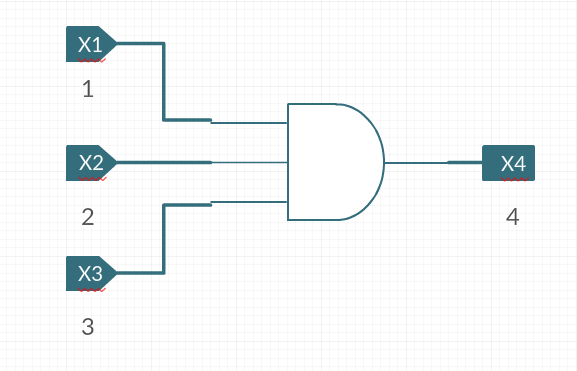
\includegraphics[width=0.3\textwidth]{3-input-and-ul.png}} 
	\subfloat[]{\label{fig:and-ur}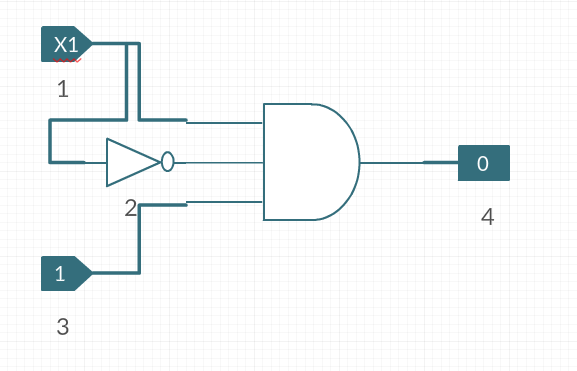
\includegraphics[width=0.3\textwidth]{3-input-and-ur.png}} 
	
	\subfloat[]{\label{fig:and-ll}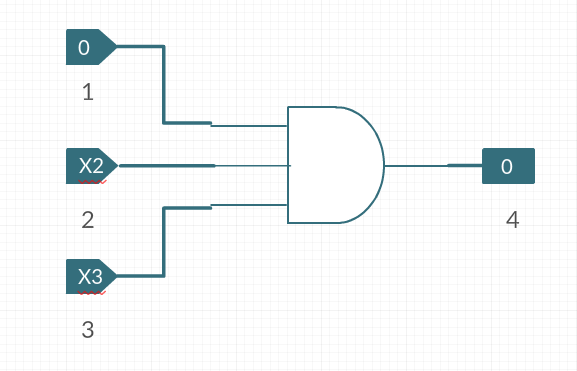
\includegraphics[width=0.3\textwidth]{3-input-and-ll.png}}
	\subfloat[]{\label{fig:and-lr}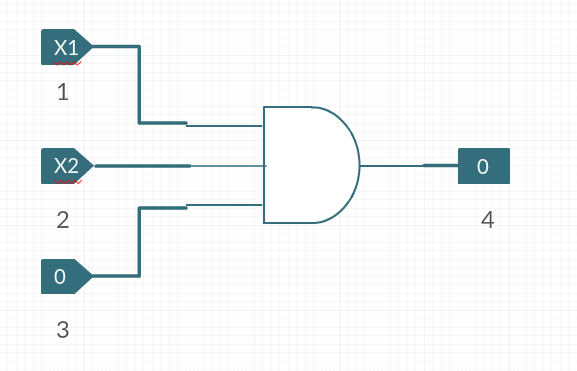
\includegraphics[width=0.3\textwidth]{3-input-and-lr.png}}
	\label{fig:and-group}
	\caption[Multi-input AND Gates]{Various Multi-input AND Gate Configurations}
\end{figure}

\begin{figure}[h!]
	\centering
	\subfloat[]{\label{fig:or-ul}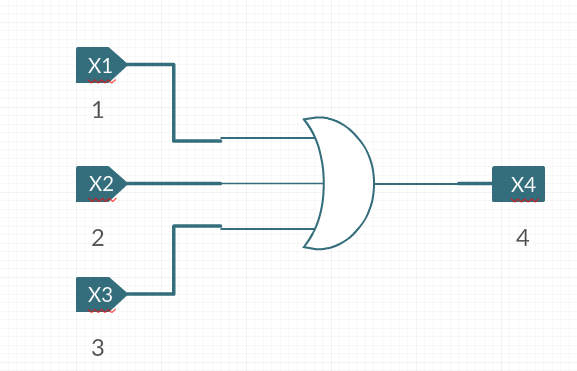
\includegraphics[width=0.3\textwidth]{3-input-or-ul.png}}
	\subfloat[]{\label{fig:or-ur}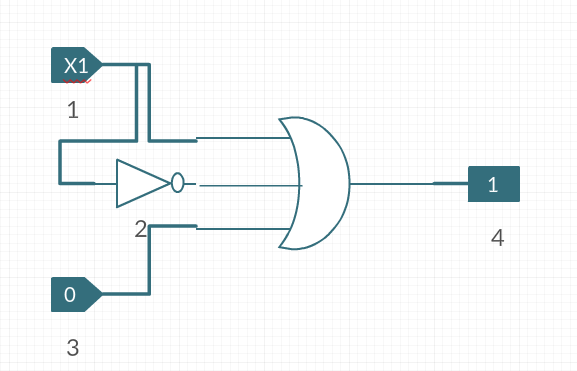
\includegraphics[width=0.3\textwidth]{3-input-or-ur.png}}
	
	\subfloat[]{\label{fig:or-ll}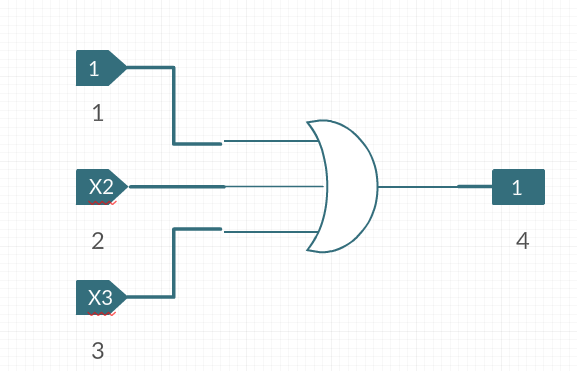
\includegraphics[width=0.3\textwidth]{3-input-or-ll.png}}
	\subfloat[]{\label{fig:or-lr}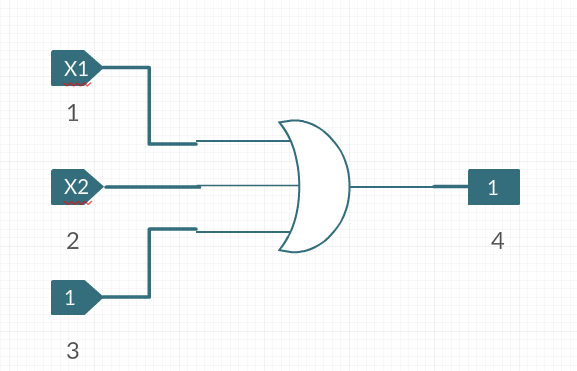
\includegraphics[width=0.3\textwidth]{3-input-or-lr.png}}
	\label{fig:or-group}
	\caption[Multi-input OR Gates]{Various Multi-input OR Gate Configurations}
\end{figure}

\section{XOR}\label{sec:xor}

XOR gates came with their own complications when converting to multi-input as opposed to dual input. For starters, XOR gates do not have a controlling value that allows the simulator to simply pass on that value, so all inputs must always be checked. Furthermore, using the implementation that was created for 2-input gates, the order of the inputs would matter. This is because after two unique X's were encountered, such as in \cref{fig:xor-lr}, the system would always create a new X value. To counter this, the simulator needed to keep track of all previous X values encountered, to see if they could be canceled, or to see if they should evaluate to 1, like if an X value and its inverse were encountered. This was actually solved through the use of X-Trees, which tracked X values and could be used to restore an X value if all other competing values were eliminated.

\begin{figure}[h!]
	\centering
	\subfloat[]{\label{fig:xor-ul}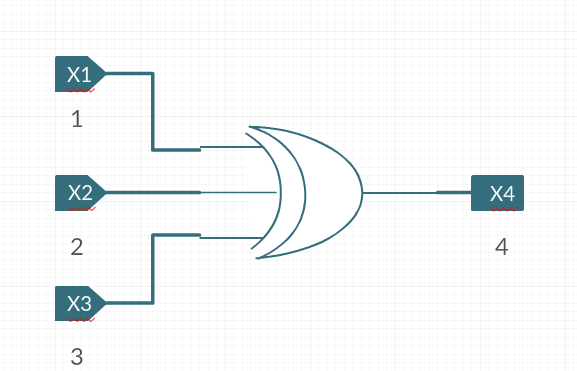
\includegraphics[width=0.3\textwidth]{3-input-xor-ul.png}}
	\subfloat[]{\label{fig:xor-ur}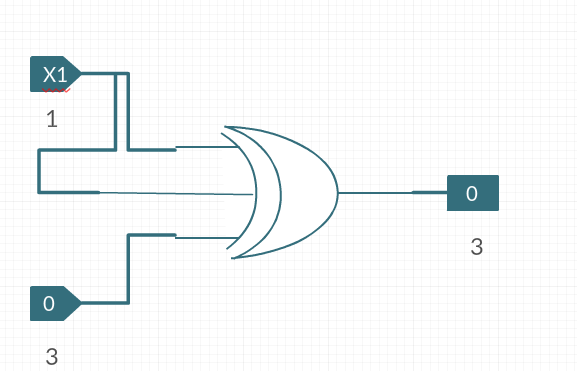
\includegraphics[width=0.3\textwidth]{3-input-xor-ur.png}}
	
	\subfloat[]{\label{fig:xor-ll}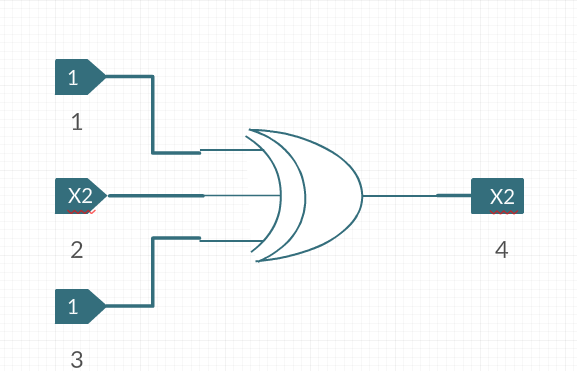
\includegraphics[width=0.3\textwidth]{3-input-xor-ll.png}}
	\subfloat[]{\label{fig:xor-lr}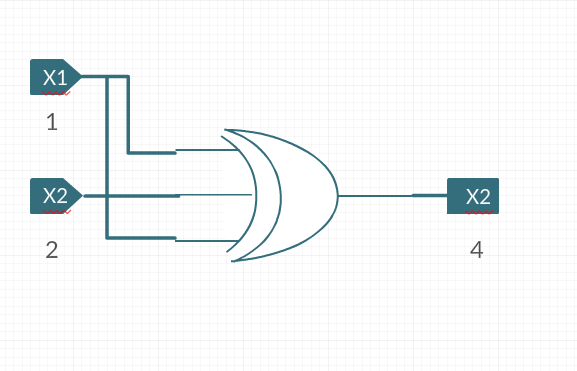
\includegraphics[width=0.3\textwidth]{3-input-xor-lr.png}}
	\label{fig:xor-group}
	\caption[Multi-input XOR Gates]{Various Multi-input XOR Gate Configurations}
\end{figure}

\singlespacing
\chapter{X-Trees}\label{sec:xtree}
\doublespacing

\section{Overview}

The X-Tree was a structure that was created to help the user track how X values mixed and evolved through a circuit. It is simply an array for each gate with a value corresponding to each X value. X\_TREE\_NA (0) represents that the current X value is not in the history of X values for the current gate. X\_TREE\_ON (1) represents that the current X value is present in the history of the current gate. X\_TREE\_OFF (2) represents that the inverse of the current X value is in the history of the current gate. These values were chosen because X\_TREE\_ON and X\_TREE\_OFF are not mutually exclusive, and in an XOR gate or an OR gate would evaluate to 1, while in an AND gate would evaluate to zero. An example of a circuit and its output from the program are given in \cref{fig:xtree-ckt,fig:sim-output}.

\begin{figure}[h]
	\centering
	\subfloat[The circuit used in the example simulation]{\label{fig:xtree-ckt}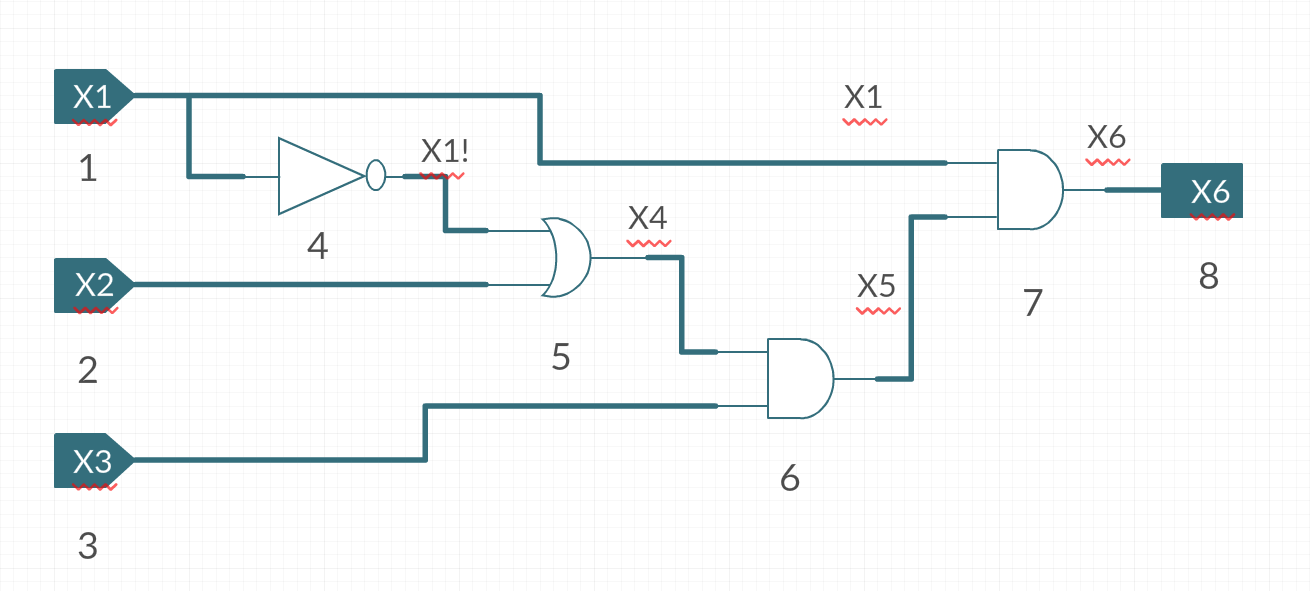
\includegraphics[width=0.5\textwidth]{xtree-circuit.png}}
	\subfloat[An example of the X-Tree output of the simulator]{\label{fig:sim-output}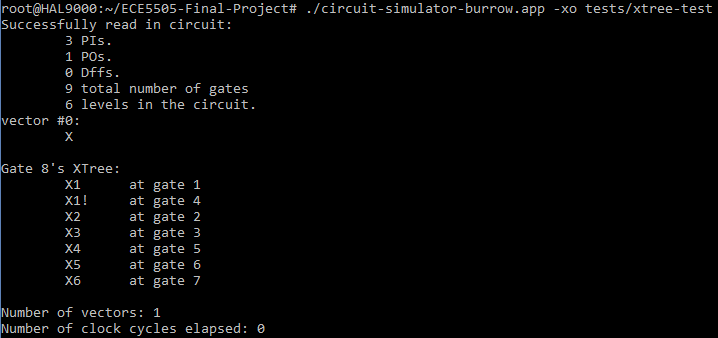
\includegraphics[width=0.5\textwidth]{sim-output.png}}	
\end{figure}

\section{Effects on Gates}\label{sec:xtree-effects}

\subsection{AND/OR}
The use of X-Trees allowed for the resolution one of the problems referenced in \cref{sec:and-or}; the problem of order of inputs. Because all of the X value inputs are now stored, by a simple check of whether the X\_TREE\_ON was present as well as the X\_TREE\_OFF value, the simulator can quickly check if both an X value and its inverse are inputs to the gate, and if so it can quickly be determined that the controlling value for the gate must occur and an output can be forced.

\subsection{XOR}
The use of X-Trees also allowed for a similar resolution in XOR gates, in which case the X value of each input was not simply added to the X-Tree of the new gate, but rather XOR'd. This allowed repeated X value inputs to be removed, and allowed the simulator to quickly and easily check if newer inputs had canceled out an older X value, de-escalating the X value if necessary.

\singlespacing
\chapter{User Interface}\label{sec:ui}
\doublespacing

The \ac{ui} was created with the intention of allowing a user to get a better understanding of the circuit through various means. The first option given to the user is the ability to view X-Trees at any gate, which allows them to track how X values change. These X-Trees include not only the X values in the tree, but also the first occurrence of each value, useful for determining where values join and evolve. A sample output of this use case can be seen in \cref{fig:sim-xtree-cmd}. The second option that was included in the \ac{ui} was the option for a user to modify the output of a gate, and see how the tree is affected. An example of this can be seen in \cref{fig:sim-gate-cmd}, in which driving a gate to value 0 forces the output to zero. This can be useful in tracing which gates are relevant or controlling in a circuit, and can be helpful in quick modifications of circuit input to try and gain ideal values. The gate control option could be evolved into an automated task for \ac{atpg}; however, I decided that this was outside of the scope of my project and what I would be able to complete in the time given.

\begin{figure}[h]
	\centering
	\subfloat[An example of the user interface and how to observe the X-Tree of any gate in the circuit]{\label{fig:sim-xtree-cmd}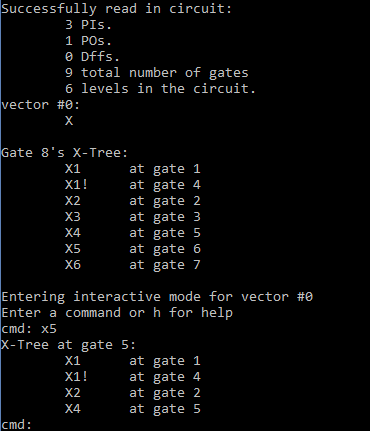
\includegraphics[width=0.4\textwidth]{sim-xtree-cmd.png}}
	\qquad
	\subfloat[An example of the user interface and how to force a value on the output of a gate]{\label{fig:sim-gate-cmd}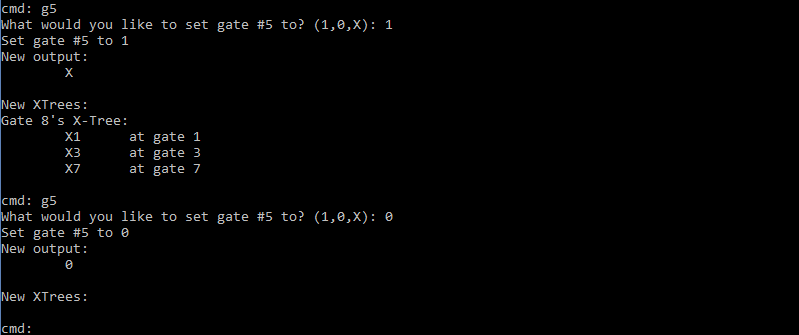
\includegraphics[width=0.4\textwidth]{sim-gate-cmd.png}}	
\end{figure}

\pdfbookmark{Bibliography}{bib}
\bibliographystyle{myIEEEtran}
\bibliography{references}

\appendix

% In LaTeX, each appendix is a "chapter"
% \chapter{Program Source}


\end{document}
